% Load the traditional font encoding before IEEEtran initializes its fonts.
% This preserves IEEEtran's Times family under both pdfLaTeX and Tectonic/XeTeX.
\RequirePackage[T1]{fontenc}
\documentclass[conference,letterpaper,10pt]{IEEEtran}
\usepackage{amsmath,amssymb}
\usepackage{graphicx,booktabs,cite,url}
\usepackage[hidelinks]{hyperref}
\graphicspath{{figures/}}
\newcommand{\HH}{\mathbb{H}}
\newcommand{\aidraft}{\par\noindent{\footnotesize\textit{AI-assisted drafting}~\cite{OpenAI2026Codex}.}\par}
\title{Quaternion Channel Grouping under Structural Compression:\\Reconstruction, Realizability, and Repair}
\author{\IEEEauthorblockN{Anonymous Authors}}
\begin{document}
\maketitle
\begin{abstract}
Structural compression of quaternion networks raises two distinct questions: which scalar channels to retain, and how to assign them to quaternion groups. We isolate assignment by keeping retained channels fixed, then measure constrained reconstruction, realization by smaller Hamilton layers and supervised recovery. In three source seeds per setting, original groups outperform fully mixed role-preserving and role-free assignments after three repair epochs: mean validation accuracy is 90.13\% versus 88.60\%/87.87\% on CIFAR-10 and 93.33\% versus 86.57\%/83.83\% on four-band EuroSAT. Actual whole-model parameter reductions are 14.48\% and 39.38\%. Repair substantially narrows the gaps, while producer-feature fitting can improve feature error yet worsen downstream reconstruction. Initialization and statistical controls show that a grouping advantage need not reflect learned quaternion entities. A bounded assignment search selects original groups; constructed synthetic examples demonstrate beneficial reassembly when component selection also changes. Together, these findings distinguish retained information, compact realizability and finite-budget recovery in quaternion compression.
\end{abstract}

\section{Introduction}
\aidraft
Quaternion networks couple four real feature channels through Hamilton weight sharing~\cite{GaudetMaida2018DeepQuaternion,Comminiello2024InductiveBiases}. Component-level compression can retain useful channels from different quaternion units, creating a practical question: how should those channels be assigned to a smaller quaternion network? Even when selected scalar information is unchanged, reassignment can alter the admissible downstream transformations and the ability of smaller upstream layers to reproduce those features.

A grouping penalty may therefore combine architectural constraints, feature statistics and incomplete recovery after compression. Distinguishing these effects matters for designing component-level pruning: reconstruction measured on a full teacher's selected features need not predict the behavior of the compact network that must generate them. Likewise, successful fine-tuning does not establish that two initial representations were interchangeable.

Figure~\ref{fig:concept} illustrates our interventions. In the real-data comparisons, retained scalar channels, output dimensions, coefficient counts and compact architecture are fixed within each source seed and compression location. We evaluate exact teacher features, physically smaller layers and equal supervised repair budgets.

The study provides three empirical contributions:
\begin{itemize}
\item A controlled separation of retained scalar information, Hamilton-constrained downstream reconstruction and compact upstream realization.
\item Physical compression results across two datasets/architectures and three source seeds, showing substantial recovery but residual grouping gaps after short repair.
\item Initialization, normalization and adaptive-search controls that distinguish a practical grouping advantage from claims of learned quaternion semantics, complemented by constructive reassembly examples.
\end{itemize}
\begin{figure*}[t]
\centering
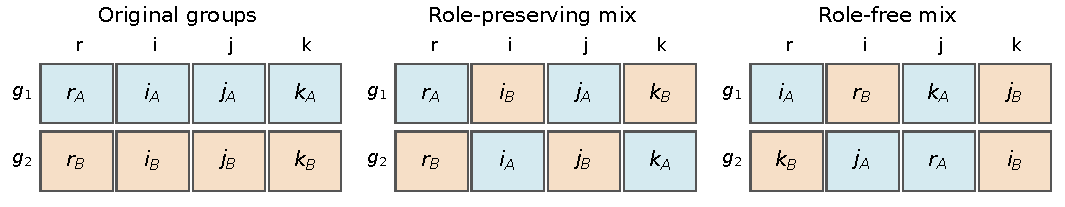
\includegraphics[width=\textwidth]{grouping_concept.pdf}
\caption{The same eight retained scalar channels assigned to two quaternion groups. Labels identify original components and source units; colors identify source units, while columns specify the new roles. Role-preserving mixing changes unit membership; role-free mixing also changes component roles. All three assignments must be realized by the same smaller Hamilton architecture.}
\label{fig:concept}
\end{figure*}

\section{Related Work}
\aidraft
Quaternion compression has been studied through targeted regularization~\cite{Vecchi2020}, transformations and pruning for audio tagging~\cite{Chaudhary2024}, and filter pruning with retraining/distillation~\cite{Singh2026}. Cross-channel weight sharing~\cite{ShahadatMaida2024CrossChannel} and hypercomplex inductive biases~\cite{Comminiello2024InductiveBiases} provide the architectural context. Our focus is the effect of assigning a fixed retained hidden scalar set to smaller Hamilton layers.

P\"oppelbaum and Schwung~\cite{PoppelbaumSchwung2025TimeCompression} study quaternion time-series compression. Their component-versus-magnitude pooling comparison operates across temporal positions; our intervention instead reassigns hidden channels and compiles smaller upstream/downstream layers. Input-channel grouping for quaternion covariance representations is also discussed in a conference abstract~\cite{Kang2026QuaternionCovarianceEEG}.

Our reconstruction uses established channel-refitting principles~\cite{He2017ChannelPruning} and hypercomplex least squares through real embeddings~\cite{VieiraValle2022ELM}. Learned grouping/shuffling~\cite{Wang2019FLGC,Zhang2021StructuredShuffle} and permutation refinement for compression~\cite{Martinez2021PermuteQuantizeFineTune} motivate the adaptive comparison. The contribution here is the controlled empirical separation, using standard ridge and projection operations.

Redundancy pruning exploits feature/filter cosine similarity~\cite{Ayinde2019}; neuron merging~\cite{Kim2020} absorbs scaling into the next layer under suitable ReLU conditions. These methods motivate distinguishing similarity from functionally valid compensation. Hamilton constraints restrict both layers in our compact pair.

Learned stitches compare representations functionally~\cite{Bansal2021ModelStitching}, while REPAIR~\cite{Jordan2023REPAIR} rescales activations for model interpolation. We use \emph{repair} for ordinary supervised fine-tuning of the compact network, distinct from that interpolation algorithm.

\section{Fixed-Information Grouping and Physical Realization}
\aidraft
\subsection{Hamilton maps and grouping interventions}
The upstream feature-producing layer is called the \emph{producer}, and the downstream feature-consuming layer the \emph{consumer}. We use component-blocked tensors and right-Hamilton multiplication. For one kernel block, the real representation is
\begin{equation}
 H(w)=\begin{bmatrix}
 w_r&-w_i&-w_j&-w_k\\
 w_i&w_r&w_k&-w_j\\
 w_j&-w_k&w_r&w_i\\
 w_k&w_j&-w_i&w_r
 \end{bmatrix}.
 \label{eq:hamilton}
\end{equation}
Entries may themselves be convolution kernels. This convention matters because quaternion multiplication is noncommutative.

Let $X$ collect patches of a fixed set of $4K$ retained scalar channels and $Y$ the full source consumer's pre-BN outputs. The original assignment groups each retained unit's four components. A permutation $P$ changes the assignment without changing the retained scalar multiset. A role-preserving assignment keeps each source component in its original $r,i,j,k$ role but can mix source units; a role-free assignment also changes roles. Affected quartets are required to contain components from multiple source units. Whole-unit reorderings are a separate invariance control.

For each assignment, the exact-feature diagnostic solves
\begin{equation}
 \widehat\theta_P=\mathop{\rm argmin}_{\theta}
 \|Y-H(\theta)PX\|_F^2+\lambda\|\theta\|_2^2.
 \label{eq:ridge}
\end{equation}
Here $\theta$ stacks the independent real Hamilton coefficients; this is zero-centered ridge, with no grouping-dependent prior. The design matrix is assembled in real arithmetic and solved using float64 moments. We fix $\lambda=10^{-3}\operatorname{mean}\operatorname{diag}(D_0^\top D_0)$ from the original assignment's design $D_0$, and reuse it across the corresponding assignments and producer variants. Reported CHECK MSE excludes the penalty.

For an unrestricted real consumer, a permutation is absorbed by an inverse permutation of its columns; a Frobenius ridge penalty is also unchanged. A numerical inverse-permutation control checks this identity, but uses a different coefficient budget and is not a competing compressed model. For the Hamilton family $\mathcal H_K$, generally $\mathcal H_KP\ne\mathcal H_K$. Thus the attainable predictions
\begin{equation}
 \mathcal D_K^{\HH}(P;X)=\{H(\theta)PX:\theta\}
\end{equation}
can depend on grouping even without learning. Whole-unit permutations preserve the family. Because $Y$ also contains contributions from omitted channels, intact groups need not give zero reconstruction error.

\subsection{A smaller producer is an additional constraint}
Gathering $PX$ from the full teacher is a diagnostic, not compact inference. A deployable student must also generate its features with a smaller Hamilton producer, scalar BN and split ReLU. For a proposed quartet, let $a_s$, $s=0,\ldots,3$, be its selected producer kernel rows. Pull each row back through the signed permutation associated with its assigned output role, giving a coefficient vector $v_s$. The Frobenius-optimal shared producer vector is
\begin{equation}
 \bar v=\tfrac14\sum_s v_s,\qquad
 C=\sum_s\|v_s-\bar v\|^2
   =\tfrac14\sum_{s<t}\|v_s-v_t\|^2.
 \label{eq:projection}
\end{equation}
This elementary projection has zero residual for original intact quartets, but arbitrary reassembly usually incurs error. Selected scalar BN parameters and buffers are copied into the assigned roles; the consumer is then refitted using the actual compact producer's activations. Deployed students contain ordinary smaller Hamilton layers, without the full teacher, runtime gathers or dense adapters.

Physical consumer error need not exceed exact-feature error: projection changes inputs and regression geometry. We report them separately, without an additive, nonnegative-cost interpretation. A local diagnostic fits only the producer kernel for 100 Adam steps on selected-feature MSE with BN fixed, then refits the consumer; it is not substituted into classification comparisons.

\section{Experimental Protocol}
\aidraft
\subsection{Data, architectures and physical budgets}
We use three existing source seeds (2026, 2027, 2028) per setting. CIFAR-10~\cite{Krizhevsky2009} uses an adapted ResNet-20~\cite{He2016ResNet}, input $(0,R,G,B)$, quaternion stage widths $8,16,32$, scalar BN, split ReLU, option-A shortcuts and a real ten-class readout. Source models were trained for 200 epochs with SGD, momentum 0.9, weight decay $10^{-4}$, five warmup epochs and scheduled learning-rate drops; selection used minimum validation cross-entropy. The split is 48,000 TRAIN, 1,000 validation and 1,000 calibration examples, with the official test set excluded from these studies.

EuroSAT~\cite{Helber2019EuroSAT} uses $64\times64$ tiles with input $(\mathrm{NIR},R,G,B)$, specifically bands B08/B04/B03/B02. A six-convolution network has quaternion widths $8,16,32$, scalar BN, split ReLU, pooling, dropout probabilities 0.1/0.2/0.3 and a real readout. The source recipe uses 50 AdamW epochs, initial learning rate $10^{-3}$ and minimum $10^{-5}$, with validation-CE checkpoint selection. Splits contain 19,600 TRAIN, 1,000 validation, 1,000 calibration and 5,400 held-out test images. Normalization uses TRAIN statistics. The NIR role is an encoding choice, not a canonical identification.

Calibration is divided into 500 FIT and 500 separate CHECK images using even/odd positions in the fixed calibration ordering. Consumer fits use all FIT spatial positions without class labels. Retention masks rank whole units by summed FIT activation second moments, retaining half the hidden units. Masks remain fixed across grouping conditions at a seed/site. We halve internal hidden widths at CIFAR blocks 0/8 and EuroSAT pairs 0/2 while preserving pair outputs and the outer graph. Parameter savings in Table~\ref{tab:budgets} are actual whole-model trainable real counts, not a claim of 50\% whole-model compression or measured acceleration.
% Generated by prepare.py; do not hand-edit numerical cells.
\begin{table}[t]
\centering\footnotesize
\caption{Actual whole-model real trainables and repair attempts per model. Successful updates: 1,125 on CIFAR; 459--461 on EuroSAT.}
\label{tab:budgets}
\begin{tabular}{lrrrr}
\toprule
Setting & Parent & Compact & Saved & Attempts \\
\midrule
CIFAR-10 & 271,594 & 232,266 & 14.48\% & 1,125 \\
EuroSAT & 73,898 & 44,794 & 39.38\% & 462 \\
\bottomrule
\end{tabular}
\end{table}


\subsection{Assignments and matched repair}
The CIFAR local study contains 23 assignments per seed/site: intact, ten predetermined fully mixed draws for each policy, and one half-mixed draw per policy, totaling 138 cases. Fifteen compact networks use intact, half-mixed and fully mixed conditions, with draw zero fixed in advance. EuroSAT classification evaluates nine networks: intact and the two fully mixed draw-zero conditions. Random draws are not independent source-training seeds, and draw zero is never selected using CHECK or validation outcomes.

Every compact model receives three epochs of supervised AdamW repair with batch size 128, learning rate $10^{-4}$ cosine-decayed to $10^{-6}$, weight decay $10^{-4}$, crop/flip augmentation and AMP. Order and augmentation streams are paired within source seed. We report final epoch three, without best-epoch selection. CIFAR has 1,125 attempted and successful updates per model. EuroSAT has 462 attempts and 459--461 successful updates per model, with 17 AMP skips in total. Equal epochs across datasets are not equal update or compute budgets; even within EuroSAT, AMP means successful counts differ slightly.

\subsection{Interpretation controls and verification}
Initialization diagnostics cross feature and consumer states, regenerating initial weights from pinned constructors/seeds. Further diagnostics sequentially recalibrate BN on 1,024 unlabelled TRAIN images, then optionally standardize scalar features using FIT moments. The standardized teacher targets are recomputed with the unchanged full consumer, so this intervention changes the diagnostic task and is not function-preserving surgery. We normalize reconstruction contrasts using CHECK target energy centered at FIT target-channel means, and inspect trained-minus-initial increments in mixed-minus-original error. Each policy averages ten draws within a source seed/site.

A separate CIFAR classification intervention recalibrates only BN running statistics in all 15 compact networks and three parents, preserving trainable parameters. Historical supervised repairs are comparators, not repairs launched from these BN-calibrated states.

Finally, a bounded adaptive CIFAR search uses two starts per site (intact and fixed free-role half-mixed), up to two rounds of 16 swaps, shortlisted by producer projection cost and private random proposals. Candidates are fit on 64 inner FIT images and scored on 64 disjoint outer FIT images; whole-network finalist combinations use teacher KL divergence with temperature two. Selected assignments are refitted on all 500 FIT images. The inherited masks already used all FIT images, so inner/outer separation is conditional on those masks.

We use local PyTorch Hamilton layers; KHNN~\cite{NiemczynowiczKycia2025} provides related hypercomplex software. Checks verify tracked parameters, gradients/updates of all four kernel components, retained sets, permutation controls, physical counts and saved predictions. Source/config/input hashes are frozen. After an archived-reference precision mismatch, EuroSAT references were regenerated in deterministic FP32 with unchanged masks/assignments; repair uses AMP. Full implementation provenance, the failed attempt and corrected protocol remain documented in the repository.

\section{Measured Results}
\aidraft
\begin{figure*}[t]
\centering
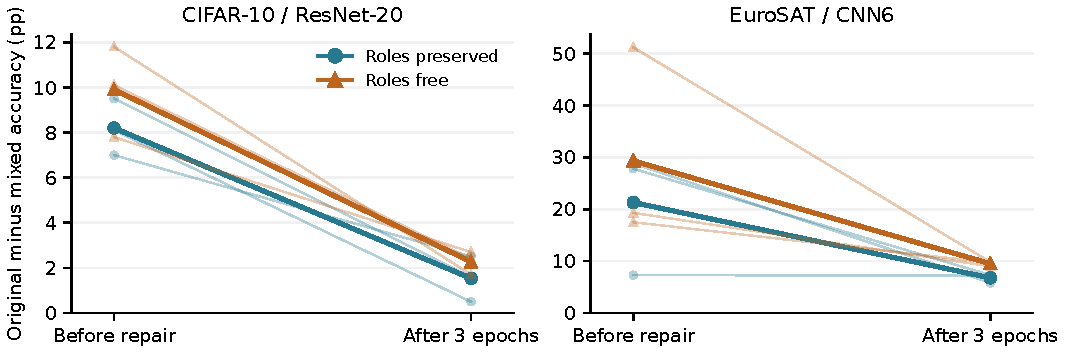
\includegraphics[width=\textwidth]{grouping_gaps.pdf}
\caption{Validation accuracy gaps for fully mixed draw-zero assignments, before and after matched three-epoch repair within each setting. Thin lines show three paired source seeds; thick lines show their descriptive mean, without confidence intervals. Both panels use percentage points but different vertical ranges. The settings also differ in architecture, input encoding, whole-model savings and repair update counts (Table~\ref{tab:budgets}). These are previously explored validation splits.}
\label{fig:gaps}
\end{figure*}
\subsection{Classification before and after repair}
Table~\ref{tab:accuracy} reports descriptive validation means and uncompressed-parent accuracy; Fig.~\ref{fig:gaps} shows paired source seeds. After repair, original grouping leads both fully mixed policies in all six paired comparisons per setting. CIFAR role/free gaps shrink from 8.20/9.90 percentage points (pp) to 1.53/2.27 pp; EuroSAT gaps shrink from 21.30/29.33 pp to 6.77/9.50 pp. Final cross-entropy also favors original grouping. CIFAR half-mixed role/free means reach 89.27\%/89.20\%, below the intact 90.13\%; all twelve mixed-versus-intact final comparisons favor intact.
% Generated by prepare.py; do not hand-edit numerical cells.
\begin{table}[t]
\centering\footnotesize
\caption{Validation accuracy (\%) and final cross-entropy, descriptive means over three source seeds. Parent rows give source accuracy only. Compact mixed conditions use the first prespecified grouping and three repair epochs.}
\label{tab:accuracy}
\begin{tabular}{lrrr}
\toprule
Grouping & Before & After & Final CE \\
\midrule
\multicolumn{4}{c}{CIFAR-10} \\
Uncompressed parent & 91.03 & --- & --- \\
Original & 87.83 & 90.13 & 0.2984 \\
Role-preserving & 79.63 & 88.60 & 0.3458 \\
Role-free & 77.93 & 87.87 & 0.3513 \\
\multicolumn{4}{c}{EuroSAT} \\
Uncompressed parent & 96.67 & --- & --- \\
Original & 79.73 & 93.33 & 0.1867 \\
Role-preserving & 58.43 & 86.57 & 0.3850 \\
Role-free & 50.40 & 83.83 & 0.4701 \\
\bottomrule
\end{tabular}
\end{table}


Repair recovers substantial accuracy in mixed models while leaving residual gaps within the tested horizon (Fig.~\ref{fig:gaps}). Larger EuroSAT gaps cannot be attributed to dataset alone: architecture, encoding, percentage savings and update budgets also change. We make no pooled cross-dataset significance claim and no equivalence claim from the smaller CIFAR gaps.

\subsection{Reconstruction is sensitive to architectural and statistical state}
In the CIFAR local study, intact grouping has lower CHECK consumer MSE than the evaluated mixed assignments on exact retained features. Physical projection can either lower or raise consumer MSE relative to that diagnostic. Producer-only fitting improves CHECK producer-feature MSE in all twelve fitted variants, yet consumer CHECK MSE worsens in four after its subsequent ridge refit. Thus closer selected-feature reproduction is not a reliable surrogate for better downstream reconstruction in these variants.
% Generated by prepare.py; do not hand-edit numerical cells.
\begin{table}[t]
\centering\footnotesize
\caption{CIFAR consumer CHECK MSE on exact retained features and physically compiled producers. Original: mean of three parents; fully mixed: mean over ten fixed draws within each of the same three parents. Raw MSE scales differ by site; draws are not independent training seeds.}
\label{tab:local}
\begin{tabular}{llrr}
\toprule
Site & Grouping & Exact & Physical \\
\midrule
Early & Original & 0.5344 & 0.5344 \\
Early & Role-preserving & 1.3066 & 1.1235 \\
Early & Role-free & 1.4675 & 1.0443 \\
Late & Original & 0.1707 & 0.1707 \\
Late & Role-preserving & 0.3967 & 0.4028 \\
Late & Role-free & 0.4107 & 0.4423 \\
\bottomrule
\end{tabular}
\end{table}


Table~\ref{tab:local} quantifies the distinction using all ten fully mixed draws per policy and site, not only classification draw zero. At the early site, physical projection lowers mean consumer MSE for both mixed policies; at the late site, it raises both means. The intact producer reproduces the selected features exactly. These results explain why the exact-feature diagnostic must not be read as a lower bound on physical reconstruction, or a kernel-projection cost as a complete downstream error model. The raw MSE scales differ between sites.

A positive mixing penalty exists at initialization in all twelve CIFAR seed/site/policy mean comparisons. Native-state penalties increase after training in all twelve, but this pattern does not survive the statistical controls (Table~\ref{tab:statistics}). After BN recalibration and marginal standardization, positive increments remain in six of twelve CIFAR and four of twelve EuroSAT comparisons. Original grouping still has lower mean error than each mixed policy at both initialization and trained states in all 24 dataset/seed/site/policy comparisons under the full control. The existence of an advantage and its amplification by training are different statements.
% Generated by prepare.py; do not hand-edit numerical cells.
\begin{table}[t]
\centering\footnotesize
\caption{Positive trained-minus-initial increments in normalized mixing penalty. Counts pair source seed, site and policy; they are not independent training replications.}
\label{tab:statistics}
\begin{tabular}{lrr}
\toprule
Diagnostic state & CIFAR-10 & EuroSAT \\
\midrule
Native & 12/12 & 11/12 \\
BN & 4/12 & 4/12 \\
BN + standardized & 6/12 & 4/12 \\
\bottomrule
\end{tabular}
\end{table}


\subsection{Constructed examples where reassembly helps}
To check that intact groups need not always be the best compression choice, an earlier synthetic diagnostic constructs two teachers with two hidden quaternion units, identical consumer coefficients across those units and complementary scalar BN biases before ReLU. Producer kernels are nearby in one teacher and independently drawn in the other. Each student has one hidden unit, 16 real trainables versus 32 in its teacher, and no runtime access to the full producer. Selection and consumer fitting use 128 FIT inputs; 1,024 independently drawn CHECK inputs measure output MSE. All 1,680 ordered selections of four distinct scalar channels are enumerated for each teacher.
% Generated by prepare.py; do not hand-edit numerical cells.
\begin{table}[t]
\centering\footnotesize
\caption{Constructed synthetic examples: held-out output MSE. Whole is the best original quartet; reassembled columns use full-teacher selected features (ideal) or the smaller producer (physical). All students store 16 real trainables versus 32 in each teacher. These examples allow the retained scalar set to change.}
\label{tab:synthetic}
\begin{tabular}{lrrr}
\toprule
Producer relation & Whole & Reassembled ideal & Physical \\
\midrule
Nearby & 0.4252 & $<10^{-12}$ & 0.0010 \\
Independent & 0.5219 & $<10^{-12}$ & 0.2865 \\
\bottomrule
\end{tabular}
\end{table}


Reassembly outperforms the best whole-unit choice in both constructed cases (Table~\ref{tab:synthetic}), but the ideal selected-feature reconstruction conceals a substantial physical error for independent producer kernels. Scalar-energy, consumer-only and physical-error selectors all choose the same role-preserving quartet $(r_0,i_1,j_0,k_1)$ in both cases. Thus these examples demonstrate feasible beneficial component reassembly, not a better selector or a benefit from changing component roles. They deliberately exploit complementary activations and, unlike the fixed-mask experiments, change the retained scalar set. They are existence examples, not representative classification evidence or a contradiction of the fixed-set results.

\subsection{BN-only recovery and adaptive grouping do not improve the control}
The CIFAR BN-only procedure closes three of twelve grouping accuracy gaps and widens nine; mean gaps widen for all four mixed conditions. For fully free mixing, the mean intact-minus-mixed gap changes from 9.90 pp natively to 11.80 pp after recalibration, compared with 2.27 pp after historical supervised repair. Intact accuracy changes from 87.83\% to 86.67\%, and free-mixed accuracy from 77.93\% to 74.87\%. Parent controls also lose 1.0 pp on average. This particular recipe fails to recover the loss; it does not rule out normalization explanations generally.

Adaptive exchange evaluates 298 unique local fits and twelve whole-network finalist combinations. All three source seeds select intact groups at both locations. Mixed-start selection MSE improves by 6.59--26.68\%, but none wins network selection. Final refits reproduce intact initializations bitwise, so their existing repaired checkpoints are reused: zero new SGD updates and zero accuracy gain. This is model reuse, not independent replication or an equivalence test.

An earlier one-seed pilot directly compared component-level selection against whole-unit pruning at 232,266 real trainables. Whole-unit, scalar-energy, role-preserving and free-role selection reached 90.4\%, 88.6\%, 90.4\% and 90.8\%, respectively. Retained sets differed and the candidate-completion mechanism favored intact groups. This exploratory comparison did not pass its prospective continuation criterion; it provides no replicated gain and is separate from the fixed-set study.

\section{Interpretation and Limitations}
\aidraft
The results support three bounded conclusions. First, preserving a scalar feature set does not preserve the representable consumer family or guarantee a realizable compact producer. Second, in the tested compact networks, the original assignments outperform the evaluated alternatives under the specified repair. Third, an original-group advantage is insufficient evidence for learned quaternion entities: it exists before training, and the training contrast depends on statistical interventions.

Random mixing is a perturbation control. The adaptive pilot tests a data-chosen alternative but only a small search around two starts. These comparisons do not establish global optimality, exclude effective regrouping methods, or demonstrate superiority over competitive compressors. No algebra or dimension comparison is implied.

There are only three source seeds per setting and one predetermined draw per full-model condition. Seed/site/policy counts are paired descriptions, not independent replications. Small observed differences do not establish practical equivalence; that requires a justified equivalence margin and appropriate uncertainty analysis~\cite{Lakens2017Equivalence}, neither of which is supplied here. The inherited masks retain complete original quartets; this isolates reassignment conditional on those masks, not optimal scalar-channel selection. Initialization is reconstructed from the pinned recipe rather than certified by an independently saved epoch-zero checkpoint. Standardization controls means/scales but changes targets and does not match covariance, sparsity or higher moments. Supervised repair changes both weights and BN statistics, and only a three-epoch horizon is tested. Local errors are not causal decompositions of classification loss.

Both validation and calibration have been inspected during earlier project development. These are exploratory results, and CHECK separation from individual fits does not make the overall research blind. No official test inference is reported for these studies. A final procedure and reporting plan must be locked, with prior split access audited, before a final test evaluation. The present draft supplies neither that evaluation nor a benchmark performance claim. We do not infer latency or FLOP gains from parameter counts.

\section{Conclusion}
\aidraft
For a fixed retained scalar set, quaternion grouping changes constrained reconstruction and physical realization, and its practical cost can persist after short supervised repair. The evaluated intact assignments outperform fully mixed alternatives in both tested settings. Initialization and statistics controls prevent interpreting this result as evidence for uniquely learned quaternion semantics, while a bounded adaptive search supplies no gain. A useful account of quaternion compression should therefore report retained information, realizable architecture and repair separately, and retain negative results that constrain the explanation.

\section*{Acknowledgment}
OpenAI Codex~\cite{OpenAI2026Codex} assisted with initial drafting of the abstract and Sections I--VII, LaTeX preparation, and table/figure-generation code using recorded experimental results. Section-opening tool citations identify drafting assistance.
\bibliographystyle{IEEEtran}
\bibliography{references}
\end{document}
